\documentclass[preprint2]{aastex}

%% preprint2 produces a double-column, single-spaced document:

%% \documentclass[preprint2]{aastex}

%% Sometimes a paper's abstract is too long to fit on the
%% title page in preprint2 mode. When that is the case,
%% use the longabstract style option.

%% \documentclass[preprint2,longabstract]{aastex}

%% If you want to create your own macros, you can do so
%% using \newcommand. Your macros should appear before
%% the \begin{document} command.
%%
%% If you are submitting to a journal that translates manuscripts
%% into SGML, you need to follow certain guidelines when preparing
%% your macros. See the AASTeX v5.x Author Guide
%% for information.

\usepackage{graphicx}
%\usepackage{caption}
%\usepackage{subcaption}
\usepackage{subfigure}
\bibliographystyle{apj}
\usepackage{natbib}
\usepackage{textcomp}

\newcommand{\tapp}{\raisebox{0.5ex}{\texttildelow}}
\newcommand{\vdag}{(v)^\dagger}
\newcommand{\myemail}{}
\newcommand{\pflux}{~photons cm$^{-2}$ s$^{-1}$}
\newcommand{\lsi}{LS~I~+61$^{\circ}$~303}
\newcommand{\gev}{\,GeV}
\newcommand{\tev}{\,TeV}

%% You can insert a short comment on the title page using the command below.


%% If you wish, you may supply running head information, although
%% this information may be modified by the editorial offices.
%% The left head contains a list of authors,
%% usually a maximum of three (otherwise use et al.).  The right
%% head is a modified title of up to roughly 44 characters.
%% Running heads will not print in the manuscript style.

\shorttitle{Bright TeV Emission from LS I +61 303}
\shortauthors{}

%% This is the end of the preamble.  Indicate the beginning of the
%% paper itself with \begin{document}.

\begin{document}

%% LaTeX will automatically break titles if they run longer than
%% one line. However, you may use \\ to force a line break if
%% you desire.

\title{Exceptionally Bright TeV Emission From the Binary \lsi{}}

%% Use \author, \affil, and the \and command to format
%% author and affiliation information.
%% Note that \email has replaced the old \authoremail command
%% from AASTeX v4.0. You can use \email to mark an email address
%% anywhere in the paper, not just in the front matter.
%% As in the title, use \\ to force line breaks.

\author{
Andy Smith\altaffilmark{1},
Anna OFdB\altaffilmark{2},
VERITAS Collaboration\altaffilmark{3}
}

%% Notice that each of these authors has alternate affiliations, which
%% are identified by the \altaffilmark after each name.  Specify alternate
%% affiliation information with \altaffiltext, with one command per each
%% affiliation.

\altaffiltext{1}{America}
\altaffiltext{2}{Germany}
\altaffiltext{3}{Everywhere}

%% Mark off your abstract in the ``abstract'' environment. In the manuscript
%% style, abstract will output a Received/Accepted line after the
%% title and affiliation information. No date will appear since the author
%% does not have this information. The dates will be filled in by the
%% editorial office after submission.

\begin{abstract}
The TeV binary system \lsi{} is known for its regular, although not entirely understood, non-thermal emission pattern, which traces the orbital period of the compact object in its 26.5 day orbit around its Be star companion. When active in the TeV regime, the system typically presents elevated emission around apastron passage with flux levels in the 5\,--\,15\,\% Crab Nebula range ($>300$\gev{}). In this article, VERITAS observations of \lsi{} taken in late 2014 are presented, in which bright TeV flares around apastron at flux levels peaking above $30\%$ of the Crab Nebula flux were detected. This is the brightest such activity ever seen in the TeV regime. The strong outbursts have rise and fall times of \tapp{}$2$ days with flux doubling times less than a day. This short acceleration time provides constraints on the nature and efficiency of the accelerating mechanism in the source.
\end{abstract}


\keywords{}

\section{Introduction}

The current generation of Imaging Atmospheric Cherenkov Telescopes (IACTs) has opened up the study of high mass X-ray binary star systems which also present TeV emission on various timescales. The class of TeV binaries is quite sparse, consisting of only a handful of sources: LS 5039 \citep{2005Sci...309..746A}, PSR B1259-63 \citep{2005A&A...442....1A}, \lsi{} \citep{Albert2006}, HESS J0632+057 \citep{2009ApJ...698L..94A}, and the newest member of the class HESS J1018-589A \citep{2015arXiv150302711H}. Of these, only the compact object of PSR B1259-63 has been firmly identified as a pulsar; there is still a large degree of ambiguity concerning the nature of the compact object within the other systems, and consequently, the fundamental setup which produces the TeV emission along with its characteristic variability on the orbital period timescale.

% For instance, the presence of a pulsar within a given TeV binary indicates that the emission in the system is generated by the shock formed at the interface between the pulsar and stellar winds. The orbital variability is therefore driven principally by the varying density of the stellar wind that the pulsar encounters in its orbit. In the case of a black hole companion, the emission is driven by an accretion-powered jet.

%Modeling of the emission from these objects has driven a very active field with models falling into both of the above categories (binary pulsar vs microquasar), as well as utilizing both leptonic and hadronic emission scenarios. As more ``direct'' attempts to measure the nature of the systems in question have yet to yield decisive information (for example, constraining the inclination angle of viewing to narrow the compact mass down to rule out a black hole) the way forward appears to be further monitoring of the systems across the spectrum in the hopes of discovering some observational feature that would firmly identify these systems and the basic interacting parts within them. 

The orbital periods of these objects vary from several days (LS 5039) to several years (PSR B129-63), and as a result, the various sources may only present short windows during which they can be studied in the TeV regime. Of the TeV binaries, \lsi{} is the only known source in the Northern Hemisphere which has a short enough orbital period (26.5 days) to allow for regular study with TeV instruments. This has made it an excellent target for Northern Hemisphere TeV observatories. 

\lsi{}, located at a distance of \tapp{}$2$ kpc, is composed of a B0 Ve star and a compact object \citep{HandC1981, Casares2005}. The observed radio to TeV emission is variable and modulated with a period of $P \approx 26.5$ days, believed to be associated with the orbital structure of the binary system \citep{Albert2006, Esposito2007, VERITASLSIDetection, Abdo2009, LiXray, 2015A&A...575L...9M}. Radial velocity measurements show the orbit to be elliptical $e = 0.537\pm0.034$, with periastron occurring around phase $\phi=0.275$, apastron at $\phi=0.775$, superior conjunction at $\phi=1.081$ and inferior conjunction at $\phi=0.313$ \citep{Aragona2009}. The periastron distance between the star and the compact object is estimated at $2.84 \times 10^{12}$\,cm (0.19\,AU), and the apastron distance at $9.57 \times 10^{12}$\,cm (0.64\,AU) \citep{2013A&ARv..21...64D}. However, the inclination of the system is not exactly known (it is expected to lie in the range $10^\circ$\,--\,$60^\circ$), leading to some uncertainty of the orbital parameters.

%As a TeV source, \lsi{} has presented puzzling behavior. Initial detections in 2006\,--\,2007 by both the MAGIC \citep{Albert2006} and VERITAS \citep{VERITASLSIDetection} collaborations over many orbital cycles showed the source to be a variably bright TeV source, with emission peaking around apastron passage. Subsequent observations in 2008\,--\,2010 \citep{2011ApJ...738....3A} showed no evidence for emission during these previously detected phases, instead only detecting the source at a lower TeV flux near the periastron passage of a single orbit. However, VERITAS observations taken in November\,--\,December 2011 showed the source to be highly active around apastron again \citep{2013ApJ...779...88A}, similar to the behavior observed in 2006\,--\,2007. Since 2011, observations of \lsi{} by VERITAS have only revealed typical emission levels, i.e., 5\,--\,15\% of the Crab Nebula flux, with emission peaking around apastron.

In this work, we present the results of the VERITAS campaign on \lsi{} in the Fall of 2014. During this time, VERITAS observed historically bright flares from \lsi{} around apastron, with the source exhibiting flux levels a factor of 2\,--\,3 times higher than previously seen.

\section{Observations}
The VERITAS IACT array, located at the base of Mt.\ Hopkins, AZ (1.3 km a.s.l., 31$^{\circ}$40'\,N, 110$^{\circ}$57'\,W) consists of four 12\,m diameter Davies-Cotton design optical telescopes. VERITAS is sensitive from 85\gev{} to 30\tev{}, and has the ability to detect a 1\,\% Crab Nebula source in approximately 25 hours\footnote{\url{http://veritas.sao.arizona.edu/about-veritas-mainmenu-81/veritas-specifications-mainmenu-111}}. For a full description of the hardware components and analysis methods utilized by VERITAS, see \citet{VERITAS, KiedaVTSUpgrade, VERITASLSIDetection}, and references therein.

In the 2014 season, VERITAS observations of \lsi{} were taken from October 16 (MJD 56946) to  December 12 (MJD 57003), obtaining a total of 24.7 hours of quality selected livetime. These observations covered three separate orbital periods of \lsi{}, sampling the orbital regions of $\phi = 0.5-0.2$ (see Figure~\ref{f:fig1}). Over the entire set of observations, a total of 449 excess events above background were detected, equivalent to a significance of $21\sigma$ calculated using Equation 17 of \citet{LiMa}.

\begin{figure}[ht]
\centering
%\subfigure[\label{fig1}]{
%  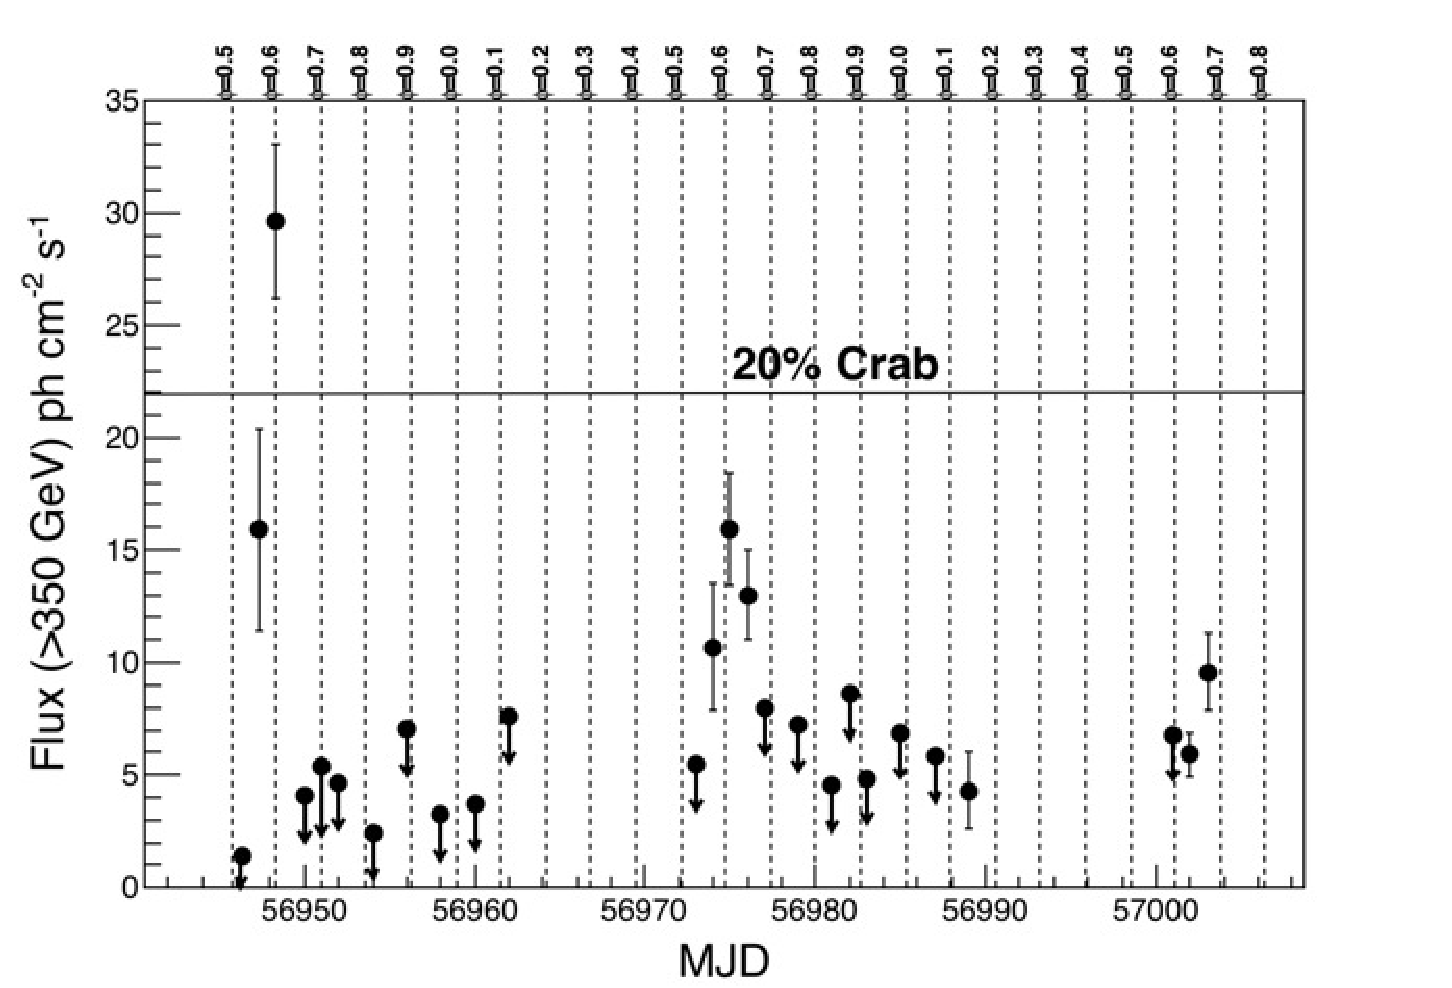
\includegraphics[width=0.5\textwidth]{./figs/Figure1-eps-converted-to.pdf}
%  %\caption{The VERITAS $>$350 GeV light curve of \lsi{} during the 2014 observation season (\textbf{VEGAS}).} 
%  %\label{fig1}
%}
%\subfigure[\label{fig1b}]{
%  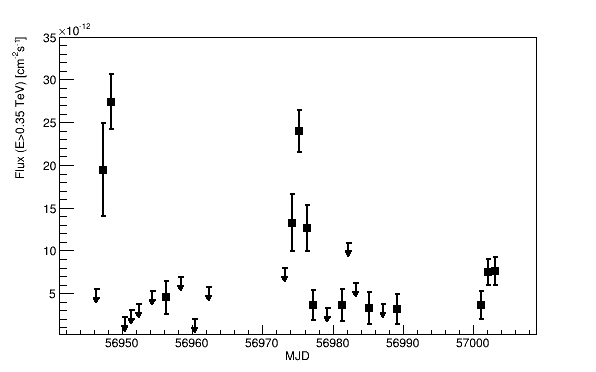
\includegraphics[width=0.5\textwidth]{figs/LSI-mod-lc-days-gt350gev.png}
%  %\caption{The VERITAS $>$350 GeV light curve of \lsi{} during the 2014 observation season (\textbf{ED}).}
%  %\label{fig1b}
%}
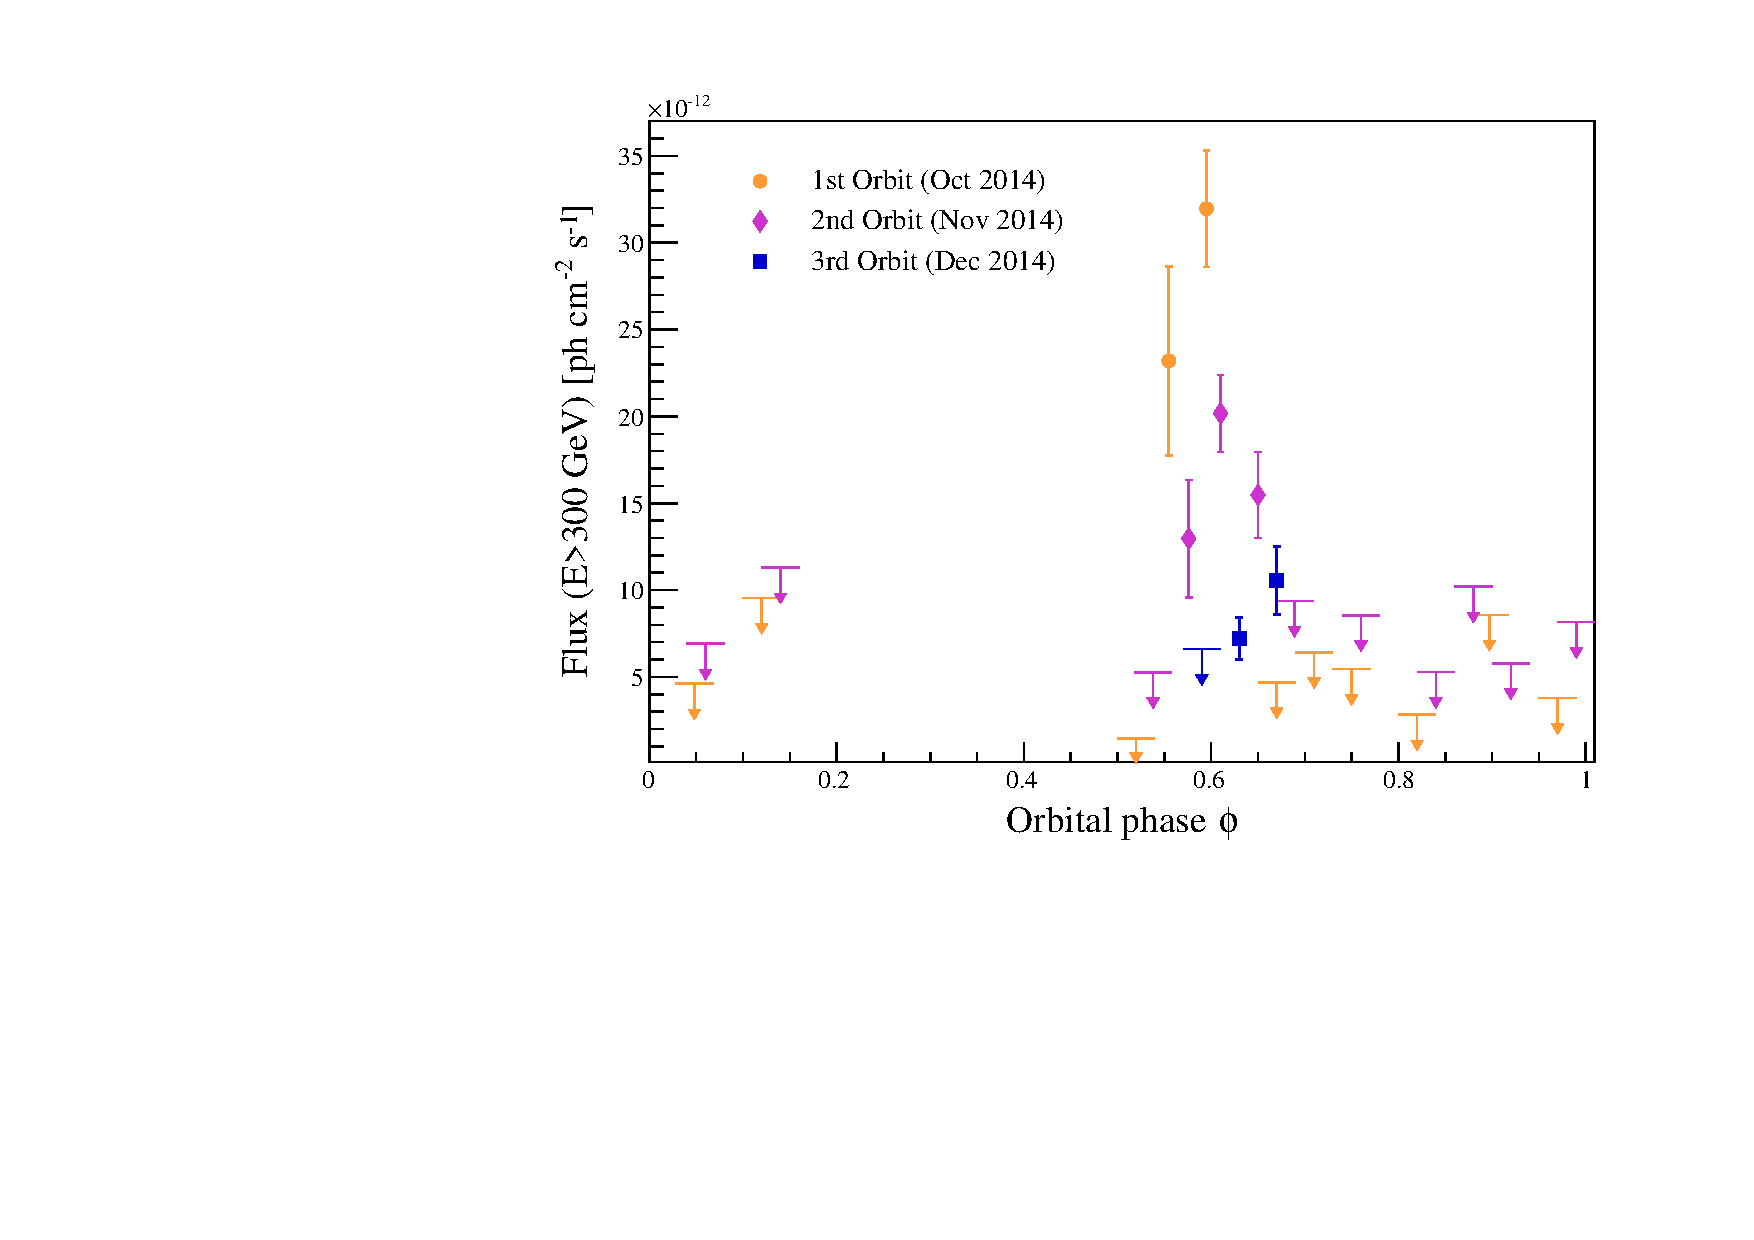
\includegraphics[width=0.5\textwidth]{./figs/fluxvphase_300.pdf}
\caption{Light curve of \lsi{} during the 2014 observation season in nightly bins. %from \textbf{VEGAS}~\subref{fig1} and \textbf{ED}~\subref{fig1b}. 
The data is shown in the different orbits observed, with the first orbit (October) shown with orange circles, the second orbit shown with purple diamonds, and the third orbit shown with blue squares. Flux upper limits at the 99\% confidence level are shown for points with $<3\,\sigma$ significance and are represented by arrows.
}
\label{f:fig1}
\end{figure}

During the first orbit observed (in October), the source presented the largest of its flares (hereafter ``F1''), beginning on 2014 October 17 (MJD 56947, $\phi = 0.55$) with emission reaching a peak of $31.9 \pm 3.4 \times10^{-12}$\pflux{} ($>$300\gev{}) on October 18 (MJD 56948). This flare peaked at approximately $30\%$ of the Crab Nebula flux in the same energy range, representing the largest flux ever detected from the source. Unfortunately, observations were limited by poor weather conditions for two nights following this peak and only recommenced on October 20 (MJD 56950), by which time the source had already quietened down. During the November observations (second orbital passage), VERITAS detected another period of high activity (``F2'') from the source at similar orbital phases ($\phi = 0.5-0.6$) with peak emission of $20.2 \pm 2.2 \times10^{-12}$\pflux{} ($>$300\gev{}) on November 14 (MJD 56975).

The rise and fall times of the flares was determined by fitting a Gaussian on top of a constant baseline to the light curve of each orbit, and also by comparing the flux on the peak night of each flare to the flux levels on different nights before and after the peak. Both F1 and F2 were found to have rise/fall times of \tapp{}$2$ days. The rapid increase in flux at the onset of F1 implies flux doubling timescales of less than a day (see Figure~\ref{f:fig1}). Similar to the findings of \cite{2013ApJ...779...88A}, a hint of nightly variability at a significance level of \tapp{}$3.5\,\sigma$ was found in F1.

Follow-up observations conducted by VERITAS during the next month (2014 December 10\,--\,12) covered the orbital phases of $\phi=0.59-0.67$ and detected the source at a lower flux level, reaching only $7.2 \pm 1.2 \times10^{-12}$\pflux{} ($>$300\gev{}) around the orbital phase at which the flares were detected in the previous orbits. The observations during this month exclude the type of peaked flaring behavior seen at the same phase range in the previous two orbital cycles, perhaps indicating some orbit-to-orbit variations in the source.

%As seen in Figure~\ref{f:fig1}, this flare is rather sharply defined: only one night before the flare began, the source was in a quescient state with a $99\%$ confidence upper limit of emission of $1.4 \times10^{-11}$\pflux{} ($>$350 GeV). \textbf{This short variability fast confirms the result of \citep{2013ApJ...779...88A}.}

During the 2014 observing season, the average differential energy spectrum of \lsi{} was consistent with past observations, i.e., the emission in the $0.3-20$\tev{} range is well fit by a power-law described by $\left( 1.70 \pm 0.69_{\mathrm{stat}} \right) \times 10^{-12} \cdot \left( \frac{E}{\mathrm{1 TeV}} \right)^{-2.35 \pm 0.32_{\mathrm{stat}}}$ cm$^{-2}$ s$^{-1}$ TeV$^{-1}$. Differential energy spectra were also extracted from F1 (October 17-18)  and F2 (November 13-15) and show a similar spectral shape, albeit with a higher normalization constant. The spectrum of F1 is described by $\left( 8.6 \pm 1.0_{\mathrm{stat}} \right) \times 10^{-12} \cdot \left( \frac{E}{\mathrm{1 TeV}} \right)^{-2.24 \pm 0.12_{\mathrm{stat}}}$ cm$^{-2}$ s$^{-1}$ TeV$^{-1}$, and the spectrum of F2 is described by $\left( 4.8 \pm 0.4_{\mathrm{stat}} \right) \times 10^{-12} \cdot \left( \frac{E}{\mathrm{1 TeV}} \right)^{-2.36 \pm 0.12_{\mathrm{stat}}}$ cm$^{-2}$ s$^{-1}$ TeV$^{-1}$. The average and flare spectra are shown in Figure~\ref{spec} along with previous spectral measurements for comparison. The highest energy gamma-ray observed during this observations was detected during F1 with an energy of \tapp{}$10$\tev{}.

\begin{figure}[ht]
\centering
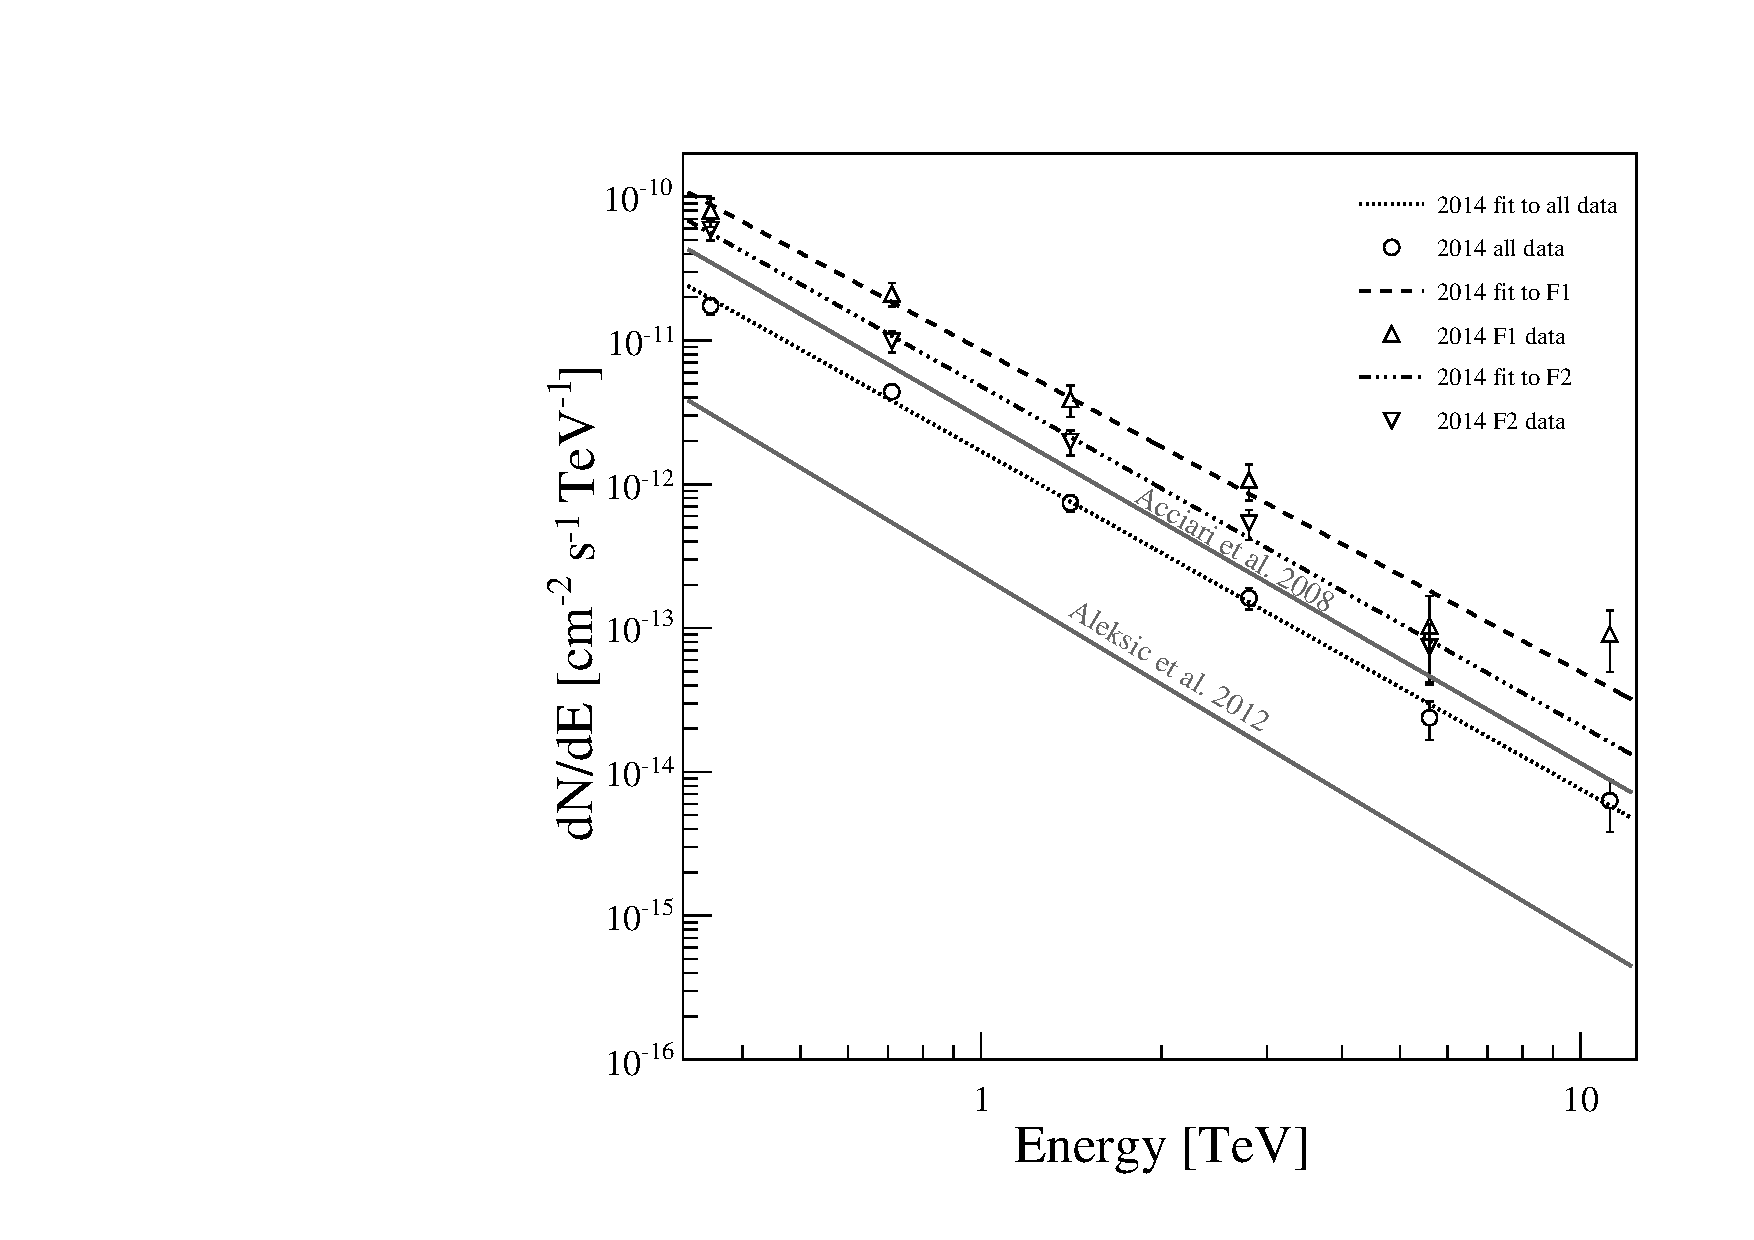
\includegraphics[width=0.5\textwidth]{figs/all_spectra_vegas.pdf}
\caption{Average and flare differential energy spectra of \lsi{} from the VERITAS 2014 observations, shown in comparison with the average spectra from \citet{VERITASLSIDetection} and \citet{Aleksic}.}
\label{spec}
\end{figure}

During these observations, the source was also monitored by \emph{Fermi}-LAT (0.1\,--\,300\gev{}), \emph{Swift}-XRT (0.2\,--\,10 keV), and both the RATAN and AMI radio instruments (4/6\,--\,15 GHz). In addition, H-alpha monitoring of the system took place with the Ritter Observatory in Toledo, Ohio (USA). After the second flare (November) was detected by VERITAS, an ATel \citep{2015VTSATEL} was released, notifying the astronomical community of the historic flux levels and triggering more intense observations with the existing multiwavelength partners, as well as additional observations with the MAGIC TeV observatory. The results of this campaign are under analysis and will be presented in an upcoming publication. 

\section{Discussion and Conclusion}
The nature of the compact object in \lsi{} is not firmly established, and emission mechanisms proposed for the system cover both a microquasar scenario, in which non-thermal process occur in the jet of an accreting compact object \citep{Massi2001,Massi2013,2015A&A...575L...9M}, and a pulsar wind shock scenario, in which particle acceleration is the result of the interaction between the stellar and the pulsar winds \citep{Dhawan2006}. In a leptonic scenario, the TeV emission is the result of inverse-Compton (IC) scattering. \citet{2008MNRAS.383..467K} provide the means to calculate model-independent limits on the magnetic field strength and the efficiency of the accelerator within an IC scenario. It is assumed that the gamma rays are produced in the system by the IC scattering of TeV electrons on stellar photons. Given the temperature $T=2.25\times10^4$\,K \citep{2013A&ARv..21...64D} of the Be star in \lsi{}, the average energy of the stellar photons is $3kT \approx 6$\,eV, and the IC scattering will take place in the deep Klein--Nishina regime in which all of the electron energy is transferred to the scattered photons. Thus, the presence of \tapp{}$10$\tev{} photons requires \tapp{}$10$\tev{} electrons in the emitter and the acceleration time must be less than the cooling time. The acceleration timescale of the electrons can be expressed as
\begin{equation}
t_{\mbox{\scriptsize{acc}}} = \eta_{\mbox{\scriptsize{acc}}} r_{\mbox{\scriptsize{L}}} c^{-1} \approx 0.1 \eta_{\mbox{\scriptsize{acc}}} E_{\mbox{\scriptsize{TeV}}} B_{\mbox{\scriptsize{G}}}^{-1} \mbox{\,s},
\label{taccel}
\end{equation}
where $r_{\mbox{\scriptsize{L}}}$ is the Larmor radius of the electron, $E_{\mbox{\scriptsize{TeV}}}$ is the energy of the electron in units of TeV, $B_{\mbox{\scriptsize{G}}}$ is the magnetic field strength in units of Gauss, and $\eta_{\mbox{\scriptsize{acc}}} > 1$ is a parameter describing the efficiency of the accelerator (in general $\eta_{\mbox{\scriptsize{acc}}} \gg 1$). The characteristic cooling time of electrons in the Klein--Nishina regime is given by
\begin{equation}
t_{\mbox{\scriptsize{KN}}} \approx 10^3 d_{13}^2 E_{\mbox{\scriptsize{TeV}}}^{0.7} \mbox{\,s},
\end{equation}
where $d_{13}$ is the distance between the emitter and the optical star in units of $10^{13}$\,cm, and the synchrotron cooling time is 
\begin{equation}
t_{\mbox{\scriptsize{sy}}} \approx 4\times10^2 B_{\mbox{\scriptsize{G}}}^{-2} E_{\mbox{\scriptsize{TeV}}}^{-1} \mbox{\,s}.
\end{equation}
Hard gamma-ray spectral indices (from $-2$ to $-2.5$) require that $t_{\mbox{\scriptsize{KN}}} < t_{\mbox{\scriptsize{sy}}}$, as IC losses in the Klein--Nishina regime allow for the electron spectra harder than $-2$ necessary to produce such gamma-ray indices. Thus, the magnetic field in the emitter is constrained by the relation
 ${B < 0.6 d_{13}^{-1} E_{\mbox{\scriptsize{TeV}}}^{-0.85} \,\mbox{\,G}}$.
This gives values of $B \lesssim 0.3$\,G at periastron and $B \lesssim 0.1$\,G at apastron, assuming that the emitter is located close to the compact object. Using these magnetic field values in Equation~\ref{taccel} gives acceleration times in the range $3 \eta_{\mbox{\scriptsize{acc}}}$\,--\,$10 \eta_{\mbox{\scriptsize{acc}}}$. For an efficient (but not extreme) accelerator with $\eta_{\mbox{\scriptsize{acc}}} \approx 50$, this results in acceleration times of a few hundred seconds, much shorter than the observed TeV variability timescales.

\citet{Paredes-Fortuny2014} present a general pulsar wind shock scenario with an inhomogeneous stellar wind in which the Be star disc is disrupted and fragments, and these fragments fall into the shock region, pushing it closer to the pulsar. The reduction in size of the pulsar wind termination shock could allow for increased acceleration efficiency on the timescale of a few hours, depending on the size and density of the disc fragments. Such a scenario could account for the exceptionally bright TeV flares and orbit-to-orbit variations seen in \lsi{}.
\vspace{2ex}

\small{
This research is supported by grants from the U.S. Department of Energy Office of Science, the U.S. National Science Foundation and the Smithsonian Institution, by NSERC in Canada, by Science Foundation Ireland (SFI 10/RFP/AST2748) and by STFC in the U.K. We acknowledge the excellent work of the technical support staff at the Fred Lawrence Whipple Observatory and at the collaborating institutions in the construction and operation of the instrument. The VERITAS Collaboration is grateful to Trevor Weekes for his seminal contributions and leadership in the field of VHE gamma-ray astrophysics, which made this study possible. A.\ O'FdB acknowledges support through the Young Investigators Program of the Helmholtz Association.
}

\bibliography{refs}


\end{document}

%%
%% End of file `sample.tex'.
